\chapter{INTRODUCTION}

Chapter 1 should provide a clear statement of the problem posed by the project, and
why the problem is of interest. It should reflect the scenario, if available. The
introduction also needs to present background information so that the reader can
understand the significance of the problem.


\section{Project Background }

\begin{itemize}
\item Provide literature review: With the aim to provide an overview of relevant research, studies, and theories related to the problem or topic addressed in the project.

\item Relevance and Importance: Why the problem is of interest and importance now; Who will use your proposed solution; State the potential impact of your project results.

\item Current State and Limitations: Describe the current situation or existing solutions and their shortcomings.

\item Transition: Conclude by bridging into the project definition and/or objectives.
\end{itemize}

\section{Project Definition}
Define the problem in terms of the technical details and features that the product, service, or process should have. These details are often set by your advisors to make sure the project is challenging and appropriate for a Capstone project. Here's how to break it down:


\subsection{Problem Statement} 
State the problem in a single sentence or a brief paragraph.


\subsection{Context and Scope}
Define the scope of the problem—what aspects it
encompasses and what it does not cover.


\subsection{Significance and Implications} Explain why solving this problem is important.
What are the potential consequences of not addressing it?


\subsection{Quantification (if any)}
If possible, quantify the problem to demonstrate its magnitude. This could involve presenting relevant statistics, data, or trends.\\


\noindent Remember to keep the definition of the problem concise, focused, and aligned with the goals of your Capstone project. It should be easy to understand and provide a clear sense of direction for the rest of the proposal.

\section{Project Objectives}
The objectives of a Capstone project outline the specific goals and outcomes you and your team aim to achieve through the project. These objectives guide your team and provide a clear focus. When writing the objectives section, make sure they are \textbf{specific, measurable, achievable, relevant, and time-bound (SMART)}. An example is given
below:
\begin{itemize}
\item \textbf{Objective 1}: [Title]
      \begin{itemize}
        \item State the first objective in clear terms.
        \item Describe what you plan to achieve with this objective.
        \item Make it specific and measurable.
      \end{itemize}
\end{itemize}

\begin{equation}\label{eq:EMC}
E = MC^2
\end{equation}


\section{Project Specifications}
Given the project objectives above, you are asked to provide the detailed technical requirements, features, and characteristics that your project must adhere to in order to meet its objectives. These include technical needs, performance expectations, design elements, functionalities, compatibility, and security measures. Specifications guide the project's development, ensuring it meets its objectives effectively and aligns with established criteria.


\begin{figure}[t]
	\centering
	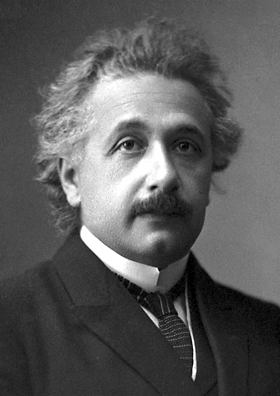
\includegraphics[width=0.5\columnwidth,trim={0cm 0.0cm 0cm 0.0cm}]{Images/Einstein.png}
% 		\vspace{-2pt}
	\caption{\small Albert Einstein is widely regarded as a genius.}
	\label{fig:queue-length}
\end{figure}



\cite{Tsebook05,SamarakoonTWC13,KeyInforcom2007}.